\documentclass[14pt, fleqn, xcolor={dvipsnames, table}]{beamer}
\usepackage[T2A]{fontenc}
\usepackage[utf8]{inputenc}
\usepackage[english,russian]{babel}
\usepackage{amssymb,amsfonts,amsmath,mathtext}
\usepackage{cite,enumerate,float,indentfirst}
\usepackage{cancel}

\usepackage{tikz}
% \usepackage{enumitem}
\usetikzlibrary{shadows}

% \usepackage{enumitem}
% \setitemize{label=\usebeamerfont*{itemize item}%
%   \usebeamercolor[fg]{itemize item}
%   \usebeamertemplate{itemize item}}

\graphicspath{{images/}}

\usetheme{Madrid}
\usecolortheme{seahorse}
\renewcommand{\CancelColor}{\color{red}}

\setbeamercolor{footline}{fg=Blue!50}
\setbeamertemplate{footline}{
  \leavevmode%
  \hbox{%
  \begin{beamercolorbox}[wd=.333333\paperwidth,ht=2.25ex,dp=1ex,center]{}%
    И. Кураленок, Н. Поваров, Яндекс
  \end{beamercolorbox}%
  \begin{beamercolorbox}[wd=.333333\paperwidth,ht=2.25ex,dp=1ex,center]{}%
    Санкт-Петербург, 2013
  \end{beamercolorbox}%
  \begin{beamercolorbox}[wd=.333333\paperwidth,ht=2.25ex,dp=1ex,right]{}%
  Стр. \insertframenumber{} из \inserttotalframenumber \hspace*{2ex}
  \end{beamercolorbox}}%
  \vskip0pt%
}
\newcommand\indentdisplays[1]{%
     \everydisplay{\addtolength\displayindent{#1}%
     \addtolength\displaywidth{-#1}}}
\newcommand{\itemi}{\item[\checkmark]}

\newenvironment{mydescription}[1]
  {\begin{list}{}%
   {\renewcommand\makelabel[1]{\color{blue}##1:\hfill}%
   \settowidth\labelwidth{\makelabel{#1}}%
   \setlength\leftmargin{\labelwidth}
   \addtolength\leftmargin{\labelsep}}}
  {\end{list}}

\title{Обзор методов оптимизации\\\small{по книге ``Методы выпукллой оптимизации'' Ю.Е.Нестерова}}
\author[]{\small{%
И.~Куралёнок,
Н.~Поваров}}
\date{}

\begin{document}

\begin{frame}
\maketitle
\small
\begin{center}
\vspace{-60pt}
\normalsize {\color{red}Я}ндекс \\
\vspace{80pt}
\footnotesize СПб, 2013
\end{center}
\end{frame}

\section{Содержание}
\begin{frame}{Содержание}
\begin{enumerate}
  \item Общая постановка задачи
  \item Области оптимизации
  \item Локальные методы безусловной оптимизации
\end{enumerate}
\end{frame}

\begin{frame}{ML и оптимизация}
  $$\begin{array}{l}
  F_0 = \arg\max_F T(F|X) \\
  F = F(x, \beta) \\
  \beta \in \mathbb{B} \subset \mathbb{R}^n \\
  \beta_0 = \arg\max_{\beta \in \mathbb{B}} T(\beta)
  \end{array}$$
\small
Кажется это задача нелинейной (в общем случае) оптимизации.
\end{frame}

\begin{frame}{Постановка задачи оптимизации}
  $$\begin{array}{l}
  \min f_0(x) \\
  f_j(x)~\le~0, j = 1...m \\
  x \in \mathbb{B} \subset \mathbb{R}^n \\
  \end{array}$$
\small
$\mathbb{B}$ - базовое допустимое множество.
$$
Q = \{x|x \in  \mathbb{B}, f_j(x) \le 0, j = 1...m\}
$$
$Q$ - допустимое множество. 
\end{frame}

\begin{frame}{Типы задач оптимизиации}
\begin{itemize}
  \item условные: $Q \subset \mathbb{R}^n$;
  \item безусловные: $Q \equiv \mathbb{R}^n$;
  \item гладкие: $f_j$ - дифференцируемы;
  \item негладкие: $\exists j: f_j$ - не дифференцируема;
  \item целочисленные: $f_i = \sin(\pi x_i) = 0, i = 1...n$;
  \item etc.
\end{itemize}
\end{frame}


\begin{frame}{Алгоритм оптимизации}
  $$
  \mathbb{P} = (\Sigma, \Omega, \Upsilon)
  $$
  Эффективность метода $M$ на задаче $P \in \mathbb{P}$ - это необходимые вычислительные затраты для приближённого решения задачи с точностью $\epsilon > 0$
\end{frame}

\begin{frame}{Общая итеративная схема}
\begin{itemize}
   \item Вход: $x_0, \epsilon > 0, t = 0, I_{-1} = \oslash$ 
   \item Основной цикл:
    \begin{enumerate}
      \item $\Sigma(x_t)$;
      \item $I_t = I_{t-1} \cup (x_t, \Omega(x_t))$;
      \item Применяем правила $M$ к $x_{t+1} = M(I_t)$;
      \item Проверяем $\Upsilon(x_{t+1}, \epsilon)$, если не выполенено, то $t=t+1$ и к шагу 1;
    \end{enumerate}
\end{itemize}
\end{frame}

\begin{frame}{Сложность метода}
\begin{itemize}
   \item Аналитическая сложность ($\mathcal{A}$): число обращений к оракулу
   \item Арифметическая сложность: общее число вычислений
\end{itemize}
\end{frame}


\begin{frame}{Виды оракулов}
\begin{itemize}
   \item нулевого порядка: $f(x_t)$ - сэмплирование, генетика, random walk, etc;
   \item первого порядка: $(f(x_t), f'(x_t))$ - градиентный спуск, TWIST, FISTA, Fobos, etc;
   \item второго порядка: $(f(x_t), f'(x_t), f''(x_t))$ - Ньютона.
\end{itemize}
\end{frame}

\begin{frame}{Оценка сложности задач глобальной оптимизации}
  $$\begin{array}{l}
  f^* = \min_{x \in \mathbb{B}} f(x) \\
  \mathbb{B} = \{x|x \in \mathbb{R}^n, x_i \in [0, 1], i = 1\ldots n\} \\
  f \in C_{L_{\infty}}^{0,0} \Leftrightarrow |f(x) - f(y)| \le L \|x - y\|_{\infty} \\
  \end{array}$$
  Будем решать равномерными сетками.
  $$\begin{array}{l}
  f(\hat{x}_t) - f^* \le \frac{L}{2t} \\
  \end{array}$$
  Зададим необходимую точность решения $\epsilon$, тогда:
  \begin{description}
    \item[$\Rightarrow$] $\mathcal{A} \le ([\frac{L}{2\epsilon}] + 2)^n$
    \item[$\Rightarrow$] а если применить \textit{сопротивляющийся оракул} то $\mathcal{A} \ge ([\frac{L}{2\epsilon}] + 2)^n$
  \end{description}
\end{frame}

\begin{frame}{Пример}
  Пусть $L = 2, n = 10, \epsilon = 0.01$ \\
  Пусть мы умеем вычислять $f$ за 100 ms \\
  $\Rightarrow \mathcal{A} \ge ([\frac{L}{2\epsilon}])^n = 10^{20}$ \\
  $\Rightarrow$ процесс сойдётся за $10^{19}$ с $\gg$ $10^{11}$ лет ($NP$-полные задачи нервно курят!) \\
  $\Rightarrow$ наверное нужно искать более эффективные методы/ограничения на задачи. \\
\end{frame}


\begin{frame}{Общая глобальная оптимизация}
\begin{mydescription}{Класс функций}
  \item[Цель] найти глобальный экстремум
  \item[Класс функций] непрерывные
  \item[Оракул] 0-2
  \item[Чего хотим] хоть какая-то сходимость к глобальному решению
  \item[Особенности] в теории - не работает. Этих кошек надо учиться готовить в каждом конкретном случае
\end{mydescription}
\end{frame}

\begin{frame}{Общая нелинейная оптимизация}
\begin{mydescription}{Класс функций}
  \item[Цель] найти локальный минимум
  \item[Класс функций] дифференцируемые
  \item[Оракул] 1-2
  \item[Чего хотим] быстро добежать до локального минимума
  \item[Особенности] множество решений, не всегда работает на больших размерностях
\end{mydescription}
\end{frame}

\begin{frame}{Выпуклая оптимизация}
\begin{mydescription}{Класс функций}
  \item[Цель] найти глобальный минимум
  \item[Класс функций] выпуклые функции
  \item[Оракул] 1
  \item[Чего хотим] приемлемую скорость сходимости к минимуму
  \item[Особенности] ограниченная размерность, тяжело привести задачу к выпуклой
\end{mydescription}
\end{frame}

\begin{frame}{Полиномиальные методы внутренней точки}
\begin{mydescription}{Класс функций}
  \item[Цель] найти глобальный минимум
  \item[Класс функций] выпуклые множества $Q$, функции с явно заданной структурой
  \item[Оракул] 2
  \item[Чего хотим] быструю сходимость к глобальному миниммуму, скорость может зависеть от структуры
  \item[Особенности] практически неограниченная размерность, задача рассматривается как белый ящик, над target функцией надо работать
\end{mydescription}
\end{frame}


\begin{frame}{Локальная аппроксимация целевой функции Тейлором}
Будем надеяться, что в окрестности $x_t$ функция хорошо аппроксимируется:
\begin{mydescription}{Квадратично}
  \item[Линейно] $f(y) = f(x) + f'(x)(y - x) + o(\|y - x\|)$
  \item[Квадратично] $f(y) = f(x) + f'(x)^T(y - x) + \frac{1}{2}(f''(x)(y - x ))^T(y - x) + o(\|y - x\|^2)$
\end{mydescription}
Если $f \in C_{L}^{k,p}$, то можно делать какие-то выводы о сходимости.
\end{frame}

\begin{frame}{Градиентный метод I}
$$\begin{array}{l}
x_0 \in \mathbb{R}^n \\
x_{t+1} = x_t - h_t f'(x_t), t= 0,... \\
\end{array}$$
Есть много методов выбора шага $h_t$:
\begin{itemize}
  \item Последовательность не зависит от истории $\{h_t\}_{0}^{\infty}$:
  $$\begin{array}{l}
  h_t = h > 0 \\
  h_t = \frac{h}{log(t+2)} \\
  \end{array}$$
  \item Полная релаксация (градиентный спуск):
  $$
  h_t = \arg\min_{h \ge 0} f (x_t - h f'(x_t))
  $$
\end{itemize}
\end{frame}

\begin{frame}{Правило Голдштейна-Армийо}
Выберем $\alpha, \beta$ и будем искать $h_t$:%, $x_{t+1} = x_{t) - h_t f^'(x_{t})$:
\small
  $$\begin{array}{l}
  \alpha f'(x_{t})^T(x_t - x_{t+1}) \le f(x_{t}) - f(x_{t+1}) \\
  \beta f'(x_{t})^T(x_t - x_{t+1}) \ge f(x_{t}) - f(x_{t+1}) \\
  \end{array}$$
\begin{center}
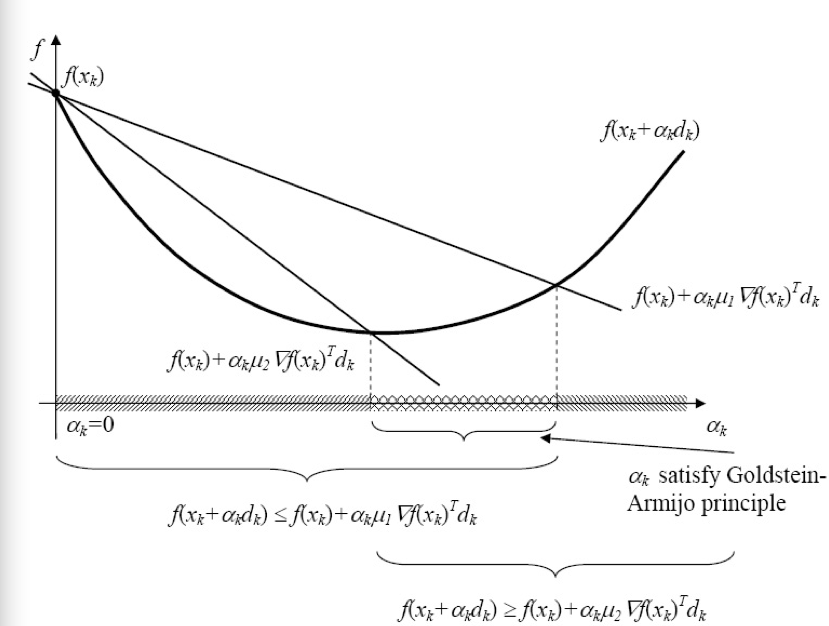
\includegraphics[height=0.6\textheight]{GoldsteinArmijo.png}
\end{center}
\end{frame}


\begin{frame}{Эффективность градиентного метода}
\small
\begin{mydescription}{Гольдштейна-Армийо}
\item[Фиксированный шаг]
$f(x_t) - f(x_{t+1}) \ge h(1 - \frac{1}{2}Lh)\|f'(x_t)\|^2$
\item[Оптимальный шаг]
$f(x_t) - f(x_{t+1}) \ge \frac{1}{2L}\|f'(x_t)\|^2$
\item[Гольдштейна-Армийо]
$f(x_t) - f(x_{t+1}) \ge \frac{2}{L}\alpha (1 - \beta) \|f'(x_t)\|^2$
\end{mydescription}
$\Rightarrow$ в общем случае $f(x_t) - f(x_{t+1}) \ge \frac{\omega}{L}\|f'(x_t)\|^2$\\
Можем получить не более чем сходимость производных (без ограниченний на гессиан):
$$\Rightarrow \min_t g_{t} \le \frac{1}{\sqrt{N+1}} \left(\frac{1}{\omega}L(f(x_0) - f^*)\right)^{\frac{1}{2}}$$
В общем случае градиентные методы умеют сходиться не к минимуму, а к стационарной точке!
\end{frame}

\begin{frame}{Метод Ньютона}
\small
$$
  x_{t+1} = x_t - (f''(x_t))^{-1}f'(x_t)
$$
Работает только близко от точки минимума (попробуйте $f(x) = \frac{x}{\sqrt{1 + x^2}}$, при начальной точке $x : |x| > 1$)!

Если:
\begin{enumerate}
   \item $f \in C_{M}^{2,2}$;
   \item гессиан положительно определен: $f''(x^*) \succeq l E, l > 0$;
   \item и мы находимся достаточно близко от оптимума $\|x_0 - x^*\| < \frac{2l}{3M}$,
\end{enumerate}
то Ньютон сходится квадратично:
$$
  \|x_{t+1} - x^*\| \le \frac{M\|x_t - x^*\|^2}{2(I - M\|x_t - x^*\|)}
$$
\end{frame}


\begin{frame}{Простые вариации метода Ньютона}
Демпфированный метод Ньютона:
$$
  x_{t+1} = x_t - h_t(f''(x_t))^{-1}f'(x_t)
$$
Гибрид:
\begin{itemize}
  \item Пойдем по градиенту;
  \item Когда окажемся близко к оптимуму, пойдем по Ньютону.
\end{itemize}
\end{frame}

\begin{frame}{Методы переменной метрики I}
\small
Предположем нам удалось найти посдедовательность $H_t$:
$$\lim_{t \to \infty} H_t = f''^{-1}$$
Тогда можно сделать:
\begin{enumerate}
  \item Выберем $x_0 \in \mathbb{R}^n$, $H_0 = E$
  \item На каждой итерации $t$:
  \begin{enumerate}
    \item $p = H_t f'(x_t)$
    \item Найдем $x_{t+1} = x_t + h_t p_t$
    \item Обновим матрицу $H_t$ на основе информации о $f(x_{t+1})$ и $f'(x_{t+1})$
  \end{enumerate}
\end{enumerate}
\end{frame}

\begin{frame}{Методы переменной метрики II}
$$
H_{t+1} \left(f'(x_{t+1}) - f'(x_t)\right) = x_{t+1} - x_{t}
$$
\small
Есть много способов удовлетворить квазиньютоновское правило, для этого введем обозначения:
$$\begin{array}{l}
  \Delta H_t = H_{t+1} - H_t,\\
  \delta_t = x_{t+1} - x_t,\\
  \gamma_t = f'(x_{t+1}) - f'(x_t)
\end{array}$$
\end{frame}
\begin{frame}{Методы переменной метрики III}
\begin{itemize}
  \item Правило одноранговой коррекции:
  $$
    \Delta H_t = \frac{(\delta_t - H_t\gamma_t)(\delta_t - H_t\gamma_t)^T}{(\delta_t - H_t\gamma_t)^T\gamma_t}
  $$
  \item Правило Давидона-Флетчера-Пауэлла(ДФП):
  $$
    \Delta H_t = \frac{\delta_t\delta_{t}^{T}}{\gamma_{t}^{T}\delta_t} - \frac{H_t\gamma_t\gamma_{t}^{T}H_t}{(H_t\gamma_t)^T\gamma_t}
  $$
  \item Правило Бройдена-Флетчера-Гольдфарба-Шенно (БФГД):
  $$\begin{array}{l}
    \Delta H_t = \frac{H_t\gamma_t\delta_{t}^{T} + \delta_t\gamma_{t}^{T}H_t}{(H_t\gamma_t)^T\gamma_t} - \beta\frac{H_t\gamma_t\gamma_{t}^{T}H_t}{(H_t\gamma_t)^T\gamma_t} \\
    \beta = 1 + \frac{\gamma_{t}^{T}\delta_t}{(H_t\gamma_t)^T\gamma_t}
  \end{array}$$
\end{itemize}
\end{frame}

\section{Выпуклая оптимизация}

\begin{frame}{ML и выпуклая оптимизация}
Часто в ML мы можем поставить задачу в терминах выпуклых функций.
$$\begin{array}{l}
  \|Ax - b\|^2 \\
  \|Ax - b\|^2 + \|x\|_1 \\
  log\frac{1}{1+e^{-t}} \\
  log\frac{1}{1+e^{c-t}} \\
\end{array}$$
\end{frame}


\begin{frame}{Пример сведения к выпуклой оптимизации}
\small
Хотим элемент классификатора $h$ из деревьев решений:
$$
\arg\min_{h \in T}\sum_{i=1}^m \log\frac{1}{1+e^{(c - \alpha h(x_i))y_i}}
$$
Деревья - зло, но как их подбирать в случае MSE мы знаем. \\
Разобьём задачку на 2 части:
$$\begin{array}{l}
  \arg\min_{\phi \in \mathbb{R}}\sum_{i=1}^mlog\frac{1}{1+e^{(c - \alpha \phi_i)y_i}} \\
  \arg\min_{h \in T}\sum_{i=1}^m(h(x_i) - \phi_i)^2
\end{array}$$
Первая часть выпуклая(на самом деле вогнутая) в $\mathbb{R}^m$, вторая - понятная. \\
$\Rightarrow$ важно научиться быстро и эффективно решать выпуклые задачи.
\end{frame}

\begin{frame}{Выпуклые функции}
\small
Есть много определений $\mathcal{F}^{1,1}$, вот некоторые из них:
$$\begin{array}{l}
  f(\alpha x + (1- \alpha)y) \le \alpha f(x) + (1-\alpha)f(y), \forall x,y ёшт \mathbb{R}^n, \alpha \in [0,1] \\
  f(y) \ge f(x) + (f'(x))^T(y-x), \forall x,y \in \mathbb{R}^n \\
  (f'(x) - f'(y))^T(x-y) \ge 0, \forall x,y \in \mathbb{R}^n 
\end{array}$$
Важнейшее для нас свойство: $f'(x) = 0 \Leftrightarrow x$ - глобальный максимум! Часто хотим чуть большего: $\mathcal{F}_L^{1,1}$, более того, сильной выпуклости $\mathcal{G}_{\mu, L}^{1,1}$:  \\
$$
f(y) \ge f(x) + (f'(x))^T(y-x) + \frac{1}{2}\mu\|x-y\|^2, \forall x,y \in \mathbb{R}^n, \mu \ge 0 
$$
\end{frame}

\begin{frame}{Класс методов}
Хотим искать решение в классе
\begin{mydescription}{Решение}
  \item [Модель] $\arg\min_{x \in \mathbb{R}^{n}}, f \in \mathcal{F}_L^{1,1}$
  \item [Оракул] локальный чёрный ящик первого порядка
  \item [Решение] $\overline{x} \in \mathbb{R}^n : f(\overline(x)) - f^* \le \epsilon$
\end{mydescription}
В этом классе решения будут лучше, чем:
$$
f(x_t) - f^* \ge \frac{3L\|x_0-x\|^2}{32(t+1)^2}
$$
при числе шагов $k < \frac{1}{2}(n-1)$.
\end{frame}

\begin{frame}{Градиентный метод}

На классе $\mathcal{F}_L^{1,1}$ и $\mathcal{G}_{\mu, L}^{1,1}$ градиентный метод с шагом $h_k=h=\frac{1}{L}$ сходится.
$$\begin{array}{l}
  f(x_t) - f^* \ge \frac{2L\|x_0-x\|^2}{t+4} \\
  f(x_t) - f^* \ge \frac{L}{2}(\frac{L - \mu}{L + \mu})^{2t}\|x_0 - x^*\|^2
\end{array}$$
Скорость сходимости - линейна на $\mathcal{F}_L^{1,1}$, а далеко не квадратична. \\
\textit{Утверждается, что релаксацией невозможно получить оптимальный метод первого порядка!}
\end{frame}

\begin{frame}{Оценивающие последовательности}
Последовательности $\{\varphi_t(x)\}_{t=0}^{\infty}$ и $\{\lambda_t(x)\}_{t=0}^{\infty}, \lambda_t \ge 0$ - \textit{оценивающие}, если $\lambda \to 0$ и $\forall x \in \mathbb{R}^n, t \ge 0$:
$$
\varphi_t(x) \ge (1- \lambda_t)f(x) + \lambda_t\varphi_0(x)
$$
Введённые последовательности хороши этим:
$$
f(x_t) - f^* \le \lambda_t(\varphi_0 - f^*) \to 0
$$

\end{frame}

\begin{frame}{Построение оценивающей последовательности}
\small
Пусть:
\begin{enumerate}
  \item $f \in \mathcal{G}_{\mu, L}^{1,1}(\mathbb{R}^n)$,
  \item $\varphi_0(x)$ - произвольная функция в $\mathbb{R}^n$,
  \item $\{y_t\}_{t=0}^{\infty}$ - произвольная последовательность в $\mathbb{R}^n$,
  \item $\{a_t\}_{t=0}^{\infty}: a_t \in (0,1), \sum_ta_t = \infty$,
  \item $\lambda_0=1$,
\end{enumerate}
тогда последовательности $\{\varphi_t(x)\}_{t=0}^{\infty}$ и $\{\lambda_t\}_{t=0}^{\infty}$:
$$\begin{array}{l}
  \lambda_{t+1} = (1 - a_t)\lambda_t, \\
  \varphi_{t+1}(x) = (1 - a_t)\varphi_t(x) + a_t(f(y_t) + f'(y_t))^T(x-y_t) + \frac{\mu}{2}\|x - y_t\|^2
\end{array}$$
оценивающие, а если $\varphi_0(x) = \varphi_0^* + \frac{\gamma_0}{2}\|x - \upsilon_0\|^2$, то и все $\varphi_0(x)$ имеют такой же вид.
\end{frame}

\begin{frame}{Общая схема оптимального метода}
\begin{enumerate}
  \item Выберем $x_0 \in \mathbb{R}^n$ и $\gamma_0 > 0$, возмьмём $\upsilon_0=x_0$.
  \item  На каждой итерации:
  \begin{enumerate}
    \item $a_t \in (0,1): La_t^2 = (1-a_t)\gamma_t + a_t\mu$, положим $\gamma_{t+1} = (1-a_t)\gamma_t + a_t\mu$
    \item Выберем  \\ 
    $y_t = \frac{a_t\gamma_t\upsilon_t + \gamma_{t+1}x_t}{\gamma_t + a_t\mu}$, \\
     вычислим $f(y_t)$ и $f'(y_t)$
    \item Найдём $x_{t+1} : f(x_{t+1}) \le f(y_{t+1}) - \frac{1}{2L}\|f'(y_t)\|^2$
    \item $\upsilon_{t+1} = \frac{(1-a_t)\gamma_t\upsilon_t + a_t\mu y_t - a_t f'(y_t)}{\gamma_{t+1}}$
  \end{enumerate}
\end{enumerate}
\end{frame}

\begin{frame}{Скорость сходимости оптимального метода}
Если всё делать по схеме, то:
$$
f(x_t) - f^* \le L\min\{(1-\sqrt{\frac{\mu}{L}})^t, \frac{4}{(t+2)^2}\}\|x_0-x^*\|^2
$$
\end{frame}

\begin{frame}{Iterative Shrinkage/Thresholding Algorithm (ISTA)}
\small
Ограничимся задачей
$$
\arg\min_{x \in \mathbb{R}^n}\|Ax - b\| + R(x)
$$
В основном интересн случай, когда $R(x) = \lambda \|x\|_1$ ($l_1$ регуляризация) или $R(x)=\lambda\|Lx\|_2$ (регуляризация Тихонова).
Заметим, что задача в случае $l_1$ негладкая.
$$\begin{array}{l}
x_{t+1} = \tau_{\lambda v_t}(x_t - 2v_tA^T(Ax_t - b)) \\
\tau_{\alpha}^i = (|x_i| - \alpha)_{+}sign(x_i)
\end{array}$$
Такая штука, являясь по сути градиентным методом сходится со скоростью:
$$
f(x_t) - f^* \ge \alpha \frac{L\|x_t - x^*\|^2}{2t}
$$
Если шаг $v_t = v$, то $\alpha=2$, если шаг брать умнее, то $\alpha<1$.
\end{frame}

\begin{frame}{Fast Iterative Shrinkage/Thresholding Algorithm (FISTA)}
Объединим ISTA и Нестерова.
\begin{enumerate}
  \item Выберем $x_0 \in \mathbb{R}^n$ и $\gamma_0 = 1$, возмьмём $y_0=x_0$.
  \item На каждой итерации
  \begin{enumerate}
    \item $x_t = \arg\min_x(R(x) + \|x - (y_{t-1} - \frac{1}{L}f'(y_{t-1}))\|^2)$
    \item $\gamma_{t+1} = \frac{1 + \sqrt{1+4\gamma_t^2}}{2}$
    \item $y_t = x_t + (\frac{\gamma_{t-1}}{\gamma_{t+1}})(x_t + x_{t-1})$
  \end{enumerate}
\end{enumerate}
Это добро сходится:
$$
f(x_t) - f^* \le \frac{\alpha L}{(t+1)^2}\|x_0 - x^*\|^2
$$
\end{frame}

\begin{frame}{Что ещё бывает?}
Область богата на исследования и приложения. Стоит почитать: Нестерова, FOBOS, etc.
\end{frame}

% \begin{frame}{Что мы сегодня узнали}

% \end{frame}

\begin{frame}{Домашняя работа}
\begin{itemize}
  \item Задания на эту неделю не будет.
  \item Результаты домашних заданий - на консультации по экзамену.
\end{itemize}
\end{frame}

\end{document}
